\documentclass[12pt,german]{article}
\usepackage{listings}
%\usepackage[utf8]{inputenc}
\usepackage{inputenc}
\usepackage{graphicx}
\usepackage{float}
\usepackage{array}
\lstset{
extendedchars=\true,
language=JAVA,
%inputencoding=utf8,
%basicstyle=\ttfamily,
%basicstyle=\ttfamily\fontsize{8}{8},
%commentstyle=\ttfamily\fontsize{8}{8},
basicstyle=\tiny;
columns=fullflexible,
%xleftmargin=5pt,
frame=single,
breaklines=true,
postbreak=\mbox{{$\hookrightarrow$}\space},
}
\renewcommand{\thesubsubsection}{\alph{subsubsection} )}
%\renewcommand{\thesubsubsection}{\thesubsection.\alph{subsubsection} )}

\begin{document}

\title{Übungsaufgaben II, SBV1 }
\author{Lisa Panholzer, Lukas Fiel}
\maketitle


\newpage
\section{Übungsaufgaben II}
\subsection{Resampling und Interpolation}
\subsubsection{Implementierung Resampling}

\subsubsection{Implementierung Bi-Lineare Interpolation}

\subsubsection{Implementierung Checker-Board}

\subsection{Klassifizierung mittels Kompression}
\subsubsection{Klassifizierung von Texten}

\textbf{Idee}
Aus Texten in 8 verschiedenen Sprachen soll mittels Kompression eine Klassifizierung stattfinden. Dazu wurden folgende Datensätze vorbereitet:

\begin{itemize}
	\item Abstract einer wissenschaftlichen Arbeit. Diese hatte den Vorteil dass es eine deutsche und englische Übersetzung gab. Alle weiteren Sprachen wurden aus der englischen Version mittels \textit{google translate} generiert.
	\item Wörterbuch mit 10000 deutschen Wörtern. Dieser Datensatz wurde mittels \textit{google translate} in alle anderen Sprachen übersetzt.
	\item Die erste Seite der Datenschutzrichtlinien von Facebook. Da die Datenschutzrichtlinien in sämtlichen Sprachen abruf bar sind, konnte für alle Sprachen ein passender Datensatz gefunden werden.
	\item Die erste Seite der Datenschutzrichtlinien von Google. Auch hier waren Daten in allen Sprachen verfügbar.
	\item Ein Witz der aus dem deutschen in alle andern Sprachen übersetzt wurde.
\end{itemize}

Da nach einer Übersetzung die Texte in verschiedenen Sprachen ungleich viele Buchstaben beinhalten ist auch die Dateigröße unterschiedlich. Dies könnte eventuell rechnerisch berücksichtigt werden. Viel einfacher aber ist es, die letzten Buchstaben jedes langen Textes zu ignorieren und so eine einheitliche Länge des Textes zu gewährleisten. Dies wurde mittels eines shell-Skripts erreicht, welches die ersten $n$ Bytes eines Files speichert. So konnte für jeden Text eine Datei erzeugt werden die in allen Sprachen den selben Speicherbedarf hat. Da es um Klassifizierung geht ist der Verlust der letzten Buchstaben bzw Wörter nicht wesentlich. 

\lstinputlisting[frame=single,language=MATLAB,breaklines=true]{../cutData.sh}

Nach einer solchen Normierung der Texte können diese miteinander verglichen werden. Dazu wurde ein Programm in \textit{Octave} geschrieben, welches die Texte der einzelnen Datensätze miteinander vergleicht und in einer Matrix darstellt. 


\begin{figure}[H]
	\centering
	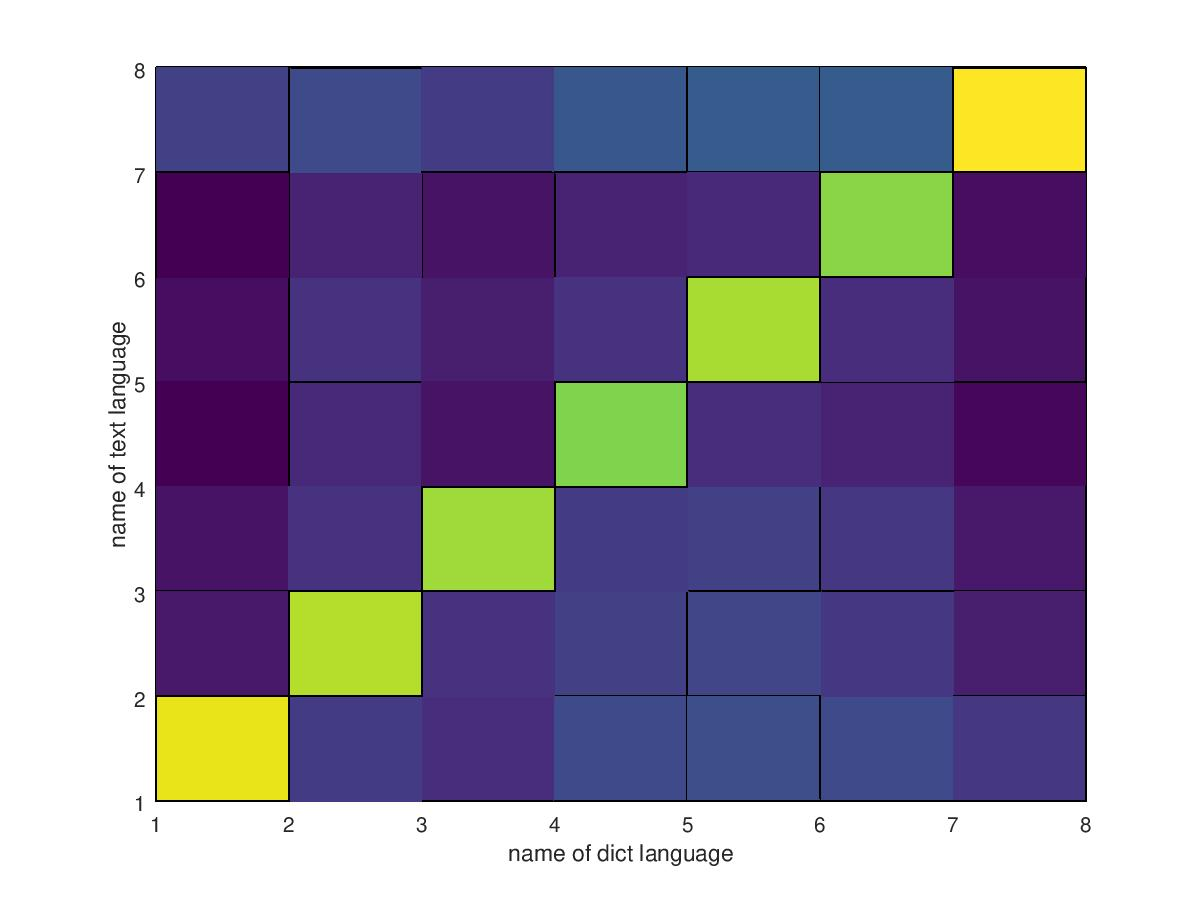
\includegraphics[width=12cm]{images/resultZipData.jpg}
	\caption{zipDataMatrix}
	\label{fig: zipDataMatrix}
\end{figure}

\lstinputlisting[frame=single,language=MATLAB,breaklines=true]{../calculateZipMatrix.m}

\subsubsection{OPTIONAL – nur für Interessierte/Experten}


\subsection{Kompression und Code-Transformation}
\subsubsection{Kompression einer Sequenz}

\subsubsection{Transformation einer Sequenz}

\subsubsection{Kompression einer Sequenz}

\subsubsection{Entropieberechnung}
\end{document}
